\documentclass{article}

\usepackage{hyperref}
\usepackage{graphicx}
\usepackage{amsmath}
\usepackage{float}



\hypersetup{
    colorlinks = true,
    linkcolor = blue,
    anchorcolor = blue
}

\graphicspath{{img/}}





\title{Parallelization of Sokoban in Java}

\author{Davide Dal Bianco \\ 2598719}

\begin{document}

\maketitle

\section{Introduction}
The Sokoban is a puzzle game where, according to some rules, the player can move his position within the board until a particular condition is met. The resolution of the game has exponential complexity, since for each state the player can move in four different directions, hence the resolution require a huge computational power. Nowadays cluster are widely used to solve complex problems, but the program must be modifiet in order to run on a cluster. In this report we will provide a possible parallelization of the game, with the main aim of describing the techniques used and measuring the performance gain.

\section{Parallel algorithm}
The provided sequential program uses a recursive function to search the solution among all the possible combinations of moves. Since the research space is infinite, it is bound by a maximum number of moves, which is gradually increased until a solution is found. It follows that the states are examined many times during the resolution. \\
There are two possible families of parallel algorithms to solve sokoban are:
\begin{itemize}
    \item A \textit{Master Worker} algorithm, where a master node creates jobs that are solved by an arbitrary number of workers.
    \item A \textit{Trasposition-Driven Scheduling} algorithm, where each node computes one move and distribute the resulting states among all the nodes according to a hash function.
\end{itemize}
However, according to the requirements, a Master Worker algorithm must be used, hence we will focus on this one only. \\
A typical Master Worker algorithm work as follows:
\begin{itemize}
    \item The master start creating the jobs and store them into a queue.
    \item The master send the jobs to the workers and the results is returned back (when needed). Some other information useful for workers may be broadcasted.
    \item The master find the final solution using the results provided by the workers.
\end{itemize}
In the sokoban, the master can start to find the solution like in the sequential version. However, every time a board reaches a maximum number of moves, the resolution of that particular board is interrupted and the board is added to the jobs queue. In this way the master can partition the global space of the solutions, in order to partition the total work among the workers. Since each partition has a different amount of work to compute, it is important that the number of jobs is much higher than the number of workers, in order to minimize the load imbalance. On the other hand, a greater number of jobs introduce a greater communication overhead. It follows that a trade off between load imbalance and communication overhead must be found. \\
In order to reflect the provided sequential algorithm, the master solve the sokoban by gradually increasing the bound. Therefore there are two options:
\begin{itemize}
    \item The current bound is less than or equal MAXHOPS and in this case only the master solve the board.
    \item The current bound is greater than MAXHOPS and in this case the master computes only the first MAXHOPS moves and the boards and the workers complete the resolution.
\end{itemize}
On the other hand, the workers are accepting new jobs from the master and, when a job is solved, the result is returned to the master. Another possible solution could be storing the cumulative result in each worker and return it back when no more jobs are available. However, workers have to notify the master they are ready for accepting a new job and therefore the communication overhead is about the same. The first solution has been chosen for its simplicity (we can think the result is piggybacked with the notification). \\


\section{Implementation}
The parallel algorithm is implemented by means of two different classes which encapsulate the master and the worker behaviour. The program must work for each number of node (even one), therefore the master node must be also a worker node. Since we have two different classes that incapsulate the two roles, the master is executed in a different thread. \\
Ibis has a built in function that elects a single node from all the joined instances. This allows to pick up a random node that will work as master. Since the number of nodes is known before the execution, we can submit it to Ibis using the java argument \texttt{-Dibis.pool.size=\#}. In this way, Ibis allows to wait until all instances have joined the pool and allows to retrieve the pool size at runtime. \\
The main of the program works as follows:
\begin{itemize}
    \item Ibis elects the server.
    \item If the current node is the server, it reads the board from the file and execute the \texttt{Server} class in a new thread.
    \item The \texttt{Worker} class is executed in the main thread.
\end{itemize}
Though the Master and the Worker are executed in two different threads, the level of parallelism is nearly zero. In fact, during the first part of the resolution workers are idle and during the second part of the resolution the master is doing IO only. For speedup measurement we can therefore assume that Master and Worker do not run concurrently. \\
In the program three different channels are used:
\begin{itemize}
    \item \textbf{greets}, used as synchronization point and to send the receive ports used by workers to accept incoming jobs.
    \item \textbf{jobSubmit}, used by the master to send the jobs to the workers.
    \item \textbf{results}, used by the workers to send the result back to the master.
\end{itemize}
In order to avoid deadlock all receive ports are opened before send ports. On the other hand, send ports are closed before receive ports.


\subsection{Master} \label{sec:master}
At the beginning, the master wait for the greeting messages from all workers containing the port used to accept new jobs. Moreover, this works as synchronization point to ensure all workers are connected and ready. \\
After the startup phase, the master start solving the board by increasing the bound. Instead of the provided recursive function, an iterative one has been used. When the list of boards is created, there are two possibilities: the current bound is less equal than MAXHOPS and the master counts the number of solved boards, or the current bound is greater than MAXHOPS and the master send the jobs to the workers in three phases:
\begin{enumerate}
    \item It send a job to each worker.
    \item When a result is returned, it send a new job to the worker.
    \item When no more jobs are available, it waits for the remaining results.
\end{enumerate}
All the solutions returned by the workers are summed. If no solutions are found the bound is incremented and the procedure is repeated until at least one solution is found. \\
At the end, the master send a null value to each worker in order to terminate it.


\subsection{Worker}
The work cycle of the workers is really easy. After the initialization of the ports, a greeting message is sent to master containing the identifier of the port used to receive jobs. After that, it starts listening for a new job. When a new one arrives, it solved and the result is sent back to the master. This message is used also to notify the master that the worker has finished the job. Now iterate the process until a null value is received.


\section{Performance measurement}
The running time of the program has been measured using system's elapsed time. For the execution of the parallel program, the IPL server run in a dedicate node. The running times have been measured for three different problem sizes:
\begin{itemize}
    \item Size 1: \texttt{t3.txt}
    \item Size 2: \texttt{t4.txt}
    \item Size 3: \texttt{t5.txt}
\end{itemize}
The file \texttt{t5.txt} wasn't provided with the test suite and it has been created ad hoc, because the provided files were too small. Each execution has been repeated four times and we took the average execution time in order to mitigate the distortion introduced by random delays. \\
\begin{figure}
\centering
\frame{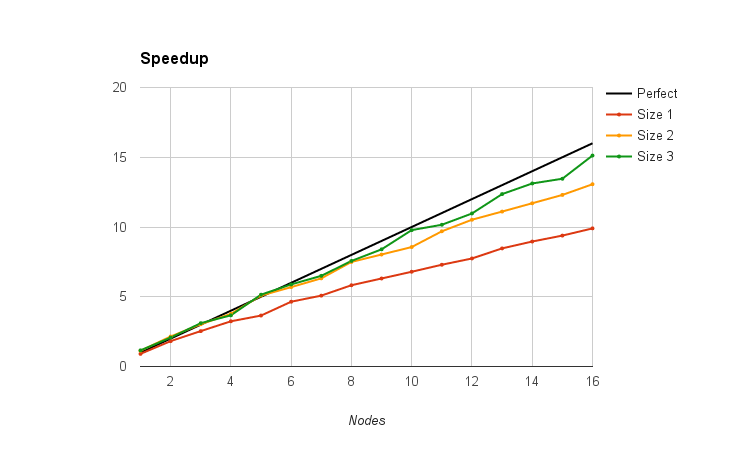
\includegraphics[width=0.8\textwidth]{speedup.png}}
\caption{Speedup for different problem sizes} \label{fig:speedup}
\end{figure}
The chart in \autoref{fig:speedup} shows the speedup for the three problem sizes. Note that the bigger the problem size, the higher the speedup. This is due to the fixed amount of work of the master. If the problem size is bigger, the workers have much more work while the overhead of communication and jobs creation do not depend on the problem size.
\begin{table}
\centering
\begin{tabular}{|l|c|c|c|}
\hline
\end{tabular}
\caption{Execution time per phase on 16 nodes} \label{tab:timeperphasecomparison}
\end{table}
In order to provide more accurate metrics, the program keep track of the duration of each phase. This is useful when optimizing the program, since bottleneck or other performance problems can be detected. \\
The vast majority of the time is spend sending the jobs to the worker. This is what we actually want, since this is the phase where the workers are working. On the other hand, the workers spend a remarkable time waiting for jobs. This time must be reduced as much as possible. Some attemps (without success) to reduce the waiting time are described in the section \nameref{sec:improvements}. \\
Overall, the measured speedup is lower than the expected one. The main reason can be found the idle time of the worker.

\section{Improvements} \label{sec:improvements}

\subsection{Overlapping jobs creation and jobs forwarding}
In section \nameref{sec:master} we described how the master creates the jobs and only later submits them to the worker. During this time interval, workers are idle and therefore much computational power is wasted. Clearly, in order to maximize performance, we must reduce the idle time as much as possible. A good solution could be using a recursive function (like a deep-first search) to compute the jobs, in order to get the first jobs sooner and be able to send them to the workers. \\
However the job creation phase is less than 0.001\% of the execution time, hence this improvement wouldn't be noticeable. For this reason it has not been implemented.


\subsection{Overlapping consecutive bounds}
Like the previous improvements, when all jobs have been sent to the workers and the master is waiting for collecting the results, some workers are idle. Though no more jobs are available, it is likely that no solution are found and the master starts creating new jobs with a greater bound. Therefore, we can exploit the idle time and use it to start executing the jobs required by the next iteration. When all results are collected there are two possibilities: if a solution is found and the jobs created are just ignored (useless work), if a solution is not found we already started the following iteration and we can continue processing it. \\
Also this improvement has not been implemented since the results collection phase consist in a minimal part of the total time. Furthermore, a more complex mechanism for collecting the results is required.


\subsection{Reducing communication latencies} \label{sec:reducinglatencies}
During its work cycle, each worker receive a job from the master, execute it and return the result back to the master. The problem is between two iteration: when the worker send back the result it must wait for another job from the master. During this gap no work is done, thus this is a possible performance loss. In order to reduce communication latencies, the next job should be sent before the worker complete the current one. In other words, at least one job should be always pending in the receive channel. This is relatively easy to implement, since it can be done by sending two messages to each worker in the first of the three sending phase. However, an unexpected performance loss has been detected. This happened due to the really small communication latencies in the cluster and the overhead caused by the higher load imbalance.

\subsection{Number of jobs instead of number of hops}
In master worker algorithms, a typical approach for creating the jobs consists in limiting the computation to a maximum number of hops (steps). This allows the master node to create many jobs that can be computed by the workers. However, in the sokoban the number of final jobs depends the starting board, since some moves are not allowed (e.g. there is a wall). Two differents board might have much different number of jobs after the same number of hops. For this reason, instead of using a fixed number of hops, we can create new jobs until the total number is greater than a constant MINJOBS. This allows to have a similar amount of jobs for each board.


\appendix

\section{Execution times}

\begin{table}[H]
\centering
\begin{tabular}{|l|c|c|c|}
\hline
Nodes & Size 1 & Size 2 & Size 3 \\ \hline
Sequential & 27474 & 75837 & 211834 \\ \hline
1 & 30.32 (0.91) & 67.20 (1.13) & 183.24 (1.16) \\ \hline 
2 & 15.11 (1.82) & 35.26 (2.15) & 102.27 (2.07) \\ \hline 
3 & 10.83 (2.54) & 25.04 (3.03) & 68.21 (3.11) \\ \hline 
4 & 8.48 (3.24) & 20.08 (3.78) & 57.73 (3.67) \\ \hline 
5 & 7.52 (3.65) & 14.93 (5.08) & 41.13 (5.15) \\ \hline 
6 & 5.92 (4.64) & 13.33 (5.69) & 36.01 (5.88) \\ \hline 
7 & 5.41 (5.08) & 12.00 (6.32) & 32.59 (6.50) \\ \hline 
8 & 4.72 (5.83) & 10.12 (7.49) & 28.00 (7.57) \\ \hline 
9 & 4.36 (6.31) & 9.45 (8.03) & 25.22 (8.40) \\ \hline 
10 & 4.05 (6.79) & 8.86 (8.56) & 21.67 (9.78) \\ \hline 
11 & 3.77 (7.29) & 7.83 (9.69) & 20.85 (10.16) \\ \hline 
12 & 3.55 (7.74) & 7.21 (10.52) & 19.31 (10.97) \\ \hline 
13 & 3.25 (8.47) & 6.83 (11.11) & 17.14 (12.36) \\ \hline 
14 & 3.07 (8.96) & 6.48 (11.70) & 16.15 (13.12) \\ \hline 
15 & 2.93 (9.38) & 6.17 (12.30) & 15.74 (13.46) \\ \hline 
16 & 2.78 (9.90) & 5.80 (13.07) & 14.01 (15.12) \\ \hline 
\end{tabular}
\caption{Execution times} \label{tab:times}
\end{table}


\end{document}